\let\negmedspace\undefined
\let\negthickspace\undefined
\documentclass[journal,12pt,onecolumn]{IEEEtran}
\usepackage{cite}
\usepackage{amsmath,amssymb,amsfonts,amsthm}
\usepackage{algorithmic}
\usepackage{graphicx}
\graphicspath{{./figs/}}
\usepackage{textcomp}
\usepackage{xcolor}
\usepackage{txfonts}
\usepackage{listings}
\usepackage{enumitem}
\usepackage{mathtools}
\usepackage{gensymb}
\usepackage{comment}
\usepackage{caption}
\usepackage[breaklinks=true]{hyperref}
\usepackage{tkz-euclide} 
\usepackage{listings}
\usepackage{gvv}                                        
                             
\usepackage[latin1]{inputenc}     
\usepackage{xparse}
\usepackage{color}                                            
\usepackage{array}                                            
\usepackage{longtable}                                       
\usepackage{calc}                                             
\usepackage{multirow}
\usepackage{multicol}
\usepackage{hhline}                                           
\usepackage{ifthen}                                           
\usepackage{lscape}
\usepackage{tabularx}
\usepackage{array}
\usepackage{float}
\newtheorem{theorem}{Theorem}[section]
\newtheorem{problem}{Problem}
\newtheorem{proposition}{Proposition}[section]
\newtheorem{lemma}{Lemma}[section]
\newtheorem{corollary}[theorem]{Corollary}
\newtheorem{example}{Example}[section]
\newtheorem{definition}[problem]{Definition}
\newcommand{\BEQA}{\begin{eqnarray}}
\newcommand{\EEQA}{\end{eqnarray}}
\newcommand{\define}{\stackrel{\triangle}{=}}
\theoremstyle{remark}
\newtheorem{rem}{Remark}


\title{\LARGE \textbf{EE - 2017}}
\author{\Large EE25BTECH11036 - M Chanakya Srinivas}

\date{}
\begin{document}
\maketitle


\begin{enumerate}

\item The matrix 
\[
A = \myvec{
\frac{3}{2} & 0 & \frac{1}{2} \\
0 & -1 & 0 \\
\frac{1}{2} & 0 & \frac{3}{2}
}
\]
has three distinct eigenvalues and one of its eigenvectors is 
\[
\myvec{ 1 \\ 0 \\ 1 }.
\]
Which one of the following can be another eigenvector of $A$?

\begin{enumerate}
\begin{multicols}{2}
\item $\myvec{ 0 \\ 0 \\ -1 }$
\item $\myvec{ -1 \\ 0 \\ 0 }$
\item $\myvec{ 0 \\ 1 \\ -1 }$
\item $\myvec{ 1 \\ 1 \\ 1 }$
\end{multicols}
\end{enumerate}

\item For a complex number $z$, 
\begin{align*}
    \lim_{z \to \infty} \frac{z^2 + 1}{z^3 + 2z - i\,(z^2+2)}
\end{align*}
is

\begin{enumerate}
\begin{multicols}{4}
    

\item $-2i$
\item $-i$
\item $i$
\item $2i$
\end{multicols}
\end{enumerate}

\item Let 
\begin{align*}
    z(t) = x(t) * y(t)
\end{align*}
 where ``*'' denotes convolution. Let $c$ be a positive real-valued constant.  
Choose the correct expression for $z(ct)$.

\begin{enumerate}
\begin{multicols}{4}
\item $c \cdot x(ct) * y(ct)$
\item $x(ct) * y(ct)$
\item $c \cdot x(t) * y(ct)$
\item $c \cdot x(ct) * y(t)$
\end{multicols}
\end{enumerate}

\item A solid iron cylinder is placed in a region containing a uniform magnetic field such that the cylinder axis is parallel to the magnetic field direction. The magnetic field lines inside the cylinder will  

\begin{enumerate}
\item be closer to the cylinder axis  
\item bend farther away from the axis  
\item remain uniform as before  
\item cease to exist inside the cylinder  
\end{enumerate}

\item Consider an electron, a neutron and a proton initially at rest and placed along a straight line such that the neutron is exactly at the center of the line joining the electron and proton. At $t=0$, the particles are released but are constrained to move along the same straight line. Which of these will collide first?

\begin{enumerate}
\begin{multicols}{2}
    

\item particles will never collide  
\item all will collide together  
\item proton and neutron  
\item electron and proton 
\end{multicols}
\end{enumerate}

\item The transfer function of a system is given by
\begin{align*}
    \frac{V_o(s)}{V_i(s)} = \frac{1-s}{1+s}.
\end{align*}
Let the output of the system be \begin{align*}
    v_o(t) = V_m \sin(\omega t + \varphi)
\end{align*}
for the input $v_i(t) = V_m \sin(\omega t)$.  
Then the minimum and maximum values of $\varphi$ (in radians) are respectively

\begin{enumerate}
\begin{multicols}{4}
    

\item $-\tfrac{\pi}{2}, \tfrac{\pi}{2}$  
\item $\tfrac{\pi}{2}, 0$  
\item $0, \tfrac{\pi}{2}$  
\item $-\pi, 0$  
\end{multicols}
\end{enumerate}

\item Consider the system with the following input-output relation
\begin{align*}
    y[n] = (1 + (-1)^n)x[n]
\end{align*}
where $x[n]$ is the input and $y[n]$ is the output. The system is

\begin{enumerate}
\begin{multicols}{2}

\item invertible and time invariant  
\item invertible and time varying  
\item non-invertible and time invariant  
\item non-invertible and time varying  
\end{multicols}
\end{enumerate}


\item A 4-pole induction machine is working as an induction generator. The generator supply frequency is $60 \,\text{Hz}$. The rotor current frequency is $5 \,\text{Hz}$. The mechanical speed of the rotor in RPM is

\begin{enumerate}
\begin{multicols}{4}
    

\item 1350  
\item 1650  
\item 1950  
\item 2250  
\end{multicols}
\end{enumerate}




\item A source is supplying a load through a 2-phase, 3-wire transmission system as shown in figure below. 
The instantaneous voltage and current in phase-a are 
\begin{align*}
    v_a = 220 \sin(100\pi t) \, V, \quad i_a = 10 \sin(100\pi t) \, A.
\end{align*}
Similarly, for phase-b, the instantaneous voltage and current are 
\begin{align*}
    v_b = 220 \cos(100\pi t) \, V, \quad i_b = 10 \cos(100\pi t) \, A.
\end{align*}
\begin{figure}[h!]
    \centering
    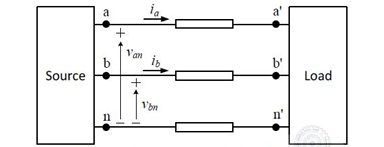
\includegraphics[width=0.5\columnwidth]{figs/9.png}
    \label{fig:placeholder}
\end{figure}
The total instantaneous power flowing from the source to the load is  

\begin{multicols}{2}
\begin{enumerate}
\item 2200 W  
\item $2200 \sin^2(100\pi t)$ W  
\item 4400 W  
\item $2200 \sin(100\pi t) \cos(100\pi t)$ W  
\end{enumerate}
\end{multicols}

\item A 3-bus power system is shown in the figure below, where the diagonal elements of Y-bus matrix are:  
$Y_{11} = -j12$ pu, $Y_{22} = -j15$ pu and $Y_{33} = -j7$ pu.  
\begin{figure}[h!]
    \centering
    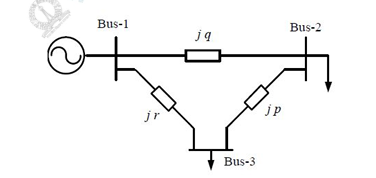
\includegraphics[width=0.5\columnwidth]{figs/10.png}
    \label{fig:placeholder}
\end{figure}
The per unit values of the line reactances $p, q, r$ and $t$ shown in the figure are  

\begin{multicols}{2}
\begin{enumerate}
\item $p = 0.2, q = -0.1, r = -0.5$  
\item $p = 0.2, q = 0.1, r = 0.5$  
\item $p = 5, q = -10, r = -2$  
\item $p = 5, q = 10, r = 2$  
\end{enumerate}
\end{multicols}

\item A closed loop system has the characteristic equation given by
\begin{align*}
    s^3 + Ks^2 + (K+2)s + 3 = 0.
\end{align*}
For this system to be stable, which one of the following conditions should be satisfied?  

\begin{multicols}{2}
\begin{enumerate}
\item $0 < K < 0.5$  
\item $0.5 < K < 1$  
\item $0 < K < 1$  
\item $K > 1$  
\end{enumerate}
\end{multicols}

\item The slope and level detector circuit in a CRO has a delay of 100 ns. The start-stop sweep generator has a response time of 50 ns. In order to display correctly, a delay line of  

\begin{multicols}{2}
\begin{enumerate}
\item 150 ns has to be inserted into the y-channel  
\item 150 ns has to be inserted into the x-channel  
\item 150 ns has to be inserted into both x and y channels  
\item 100 ns has to be inserted into both x and y channels  
\end{enumerate}
\end{multicols}

\item The Boolean expression $AB + A\bar{C} + BC$ simplifies to  

\begin{multicols}{2}
\begin{enumerate}
\item $BC + A\bar{C}$  
\item $AB + A\bar{C} + B$  
\item $AB + A\bar{C}$  
\item $AB + BC$  
\end{enumerate}
\end{multicols}

\item For the circuit shown in the figure below, assume that diodes $D_1, D_2$ and $D_3$ are ideal.  
\begin{figure}[h!]
    \centering
    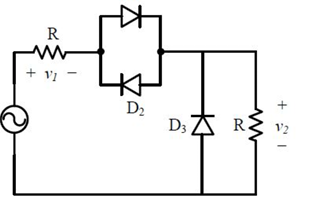
\includegraphics[width=0.5\columnwidth]{figs/14.png}
    \label{fig:placeholder}
\end{figure}
\begin{align*}
    v(t) = \pi \sin(100\pi t) \, V
\end{align*}

The DC components of voltages $v_1$ and $v_2$, respectively are  

\begin{multicols}{2}
\begin{enumerate}
\item 0 V and 1 V  
\item $-0.5$ V and 0.5 V  
\item 1 V and 0.5 V  
\item 1 V and 1 V  
\end{enumerate}
\end{multicols}




\item For the power semiconductor devices IGBT, MOSFET, Diode and Thyristor, which one of the following statements is TRUE?  

\begin{multicols}{2}
\begin{enumerate}
\item All the four are majority carrier devices.  
\item All the four are minority carrier devices.  
\item IGBT and MOSFET are majority carrier devices, whereas Diode and Thyristor are minority carrier devices.  
\item MOSFET is majority carrier device, whereas IGBT, Diode, Thyristor are minority carrier devices.  
\end{enumerate}
\end{multicols}

\item Consider 
\begin{align*}
    g(t) = 
\begin{cases}
t - \lfloor t \rfloor, & t \geq 0 \\
t - \lceil t \rceil, & \text{otherwise}
\end{cases}
\quad , \quad t \in \mathbb{R}.
\end{align*}

Here $\lfloor t \rfloor$ represents the largest integer less than or equal to $t$ and $\lceil t \rceil$ denotes the smallest integer greater than or equal to $t$. The coefficient of the second harmonic component of the Fourier series representing $g(t)$ is ______.  


\item Let 
\begin{align*}
    I = c \iint_R x y^2 \, dxdy ,
\end{align*}
where $R$ is the region shown in the figure and 
\begin{figure}[h!]
    \centering
    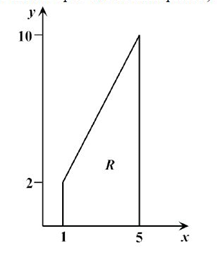
\includegraphics[width=0.5\columnwidth]{figs/17.png}
    \caption{}
    \label{fig:placeholder}
\end{figure}
\begin{align*}
    c = 6 \times 10^{-4}
\end{align*}
The value of $I$ equals (Give the answer up to two decimal places).  

\item The power supplied by the 25 V source in the figure shown below is______ W.  

\begin{figure}[h!]
    \centering
    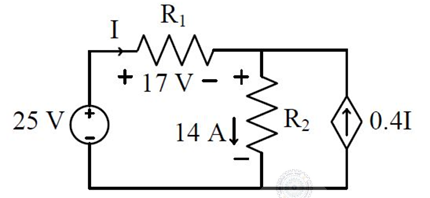
\includegraphics[width=0.5\columnwidth]{figs/18.png}
    \caption{}
    \label{fig:placeholder}
\end{figure}

\item The equivalent resistance between the terminals A and B is ______ $\ohm$.  

\begin{figure}[h!]
    \centering
    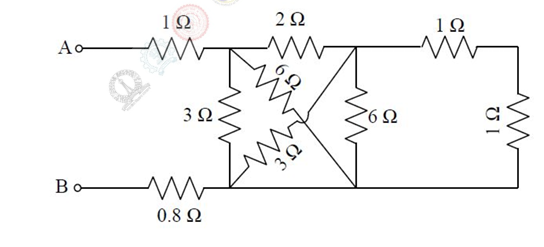
\includegraphics[width=0.5\columnwidth]{figs/19.png}
    \caption{}
    \label{fig:placeholder}
\end{figure}



\item A three-phase, 50Hz, star-connected cylindrical-rotor synchronous machine is running as a motor. 
The machine is operated from a 6.6 kV bus and draws current at unity power factor (UPF). The synchronous reactance of the motor is $8 \, \Omega$ per phase and the angle $\delta = 50^\circ$. 
The power delivered to the motor is:  
\begin{align*}
    P = \frac{EV}{X} \sin \delta
\end{align*}

\item A 10-bus power system consists of four generator buses indexed as G1, G2, G3, G4 and six load buses indexed as L1, L2, L3, L4, L5, L6. The generators G1 and G3 are connected each with a line, load bus L2 is connected to G2 via two lines, load bus L3 is connected to G4 via two lines. Each load bus has single power demand, and network is operating at an inductive reactive power balance.  
Neglecting resistance, formulate Y-bus required for solving the load flow problem using Newton-Raphson method. How many elements of Y-bus are nonzero?

\item Consider the unity feedback control system shown below. The value of $K$ that results in a phase margin of the system to be $30^\degree$ is:  
\begin{figure}[H]
    \centering
    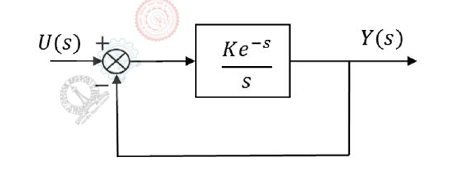
\includegraphics[width=0.5\columnwidth]{figs/22.png}
    \caption{}
    \label{fig:placeholder}
\end{figure}
\begin{align*}
    G(s) = \frac{Ke^{-s}}{s}
\end{align*}

\item The following measurements are obtained on a single phase load: $V = 220\,V$, $I = 5.0\,A$, $\phi = 0.1\%$ and $W = 55\,W \pm 2\,W$. If the power factor is calculated using these measurements, the worst case error in the calculated power factor as percent is:  

\item In the converter circuit shown below, the switches are controlled such that the load voltage $v_r(t)$ is a 400 Hz square wave.  
The RMS value of the fundamental component of $v_r(t)$ is (in volts).
\begin{figure}[H]
    \centering
    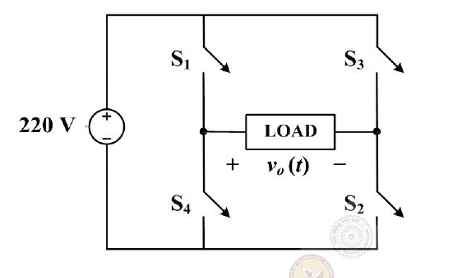
\includegraphics[width=0.5\columnwidth]{figs/24.png}
    \caption{}
    \label{fig:placeholder}
\end{figure}

\item A 3-phase voltage source inverter is supplied from a 600 V DC source as shown. For a star-connected resistive load of 20 $\Omega$ per phase, the load power for 120° device conduction is (in kW).
\begin{figure}[H]
    \centering
    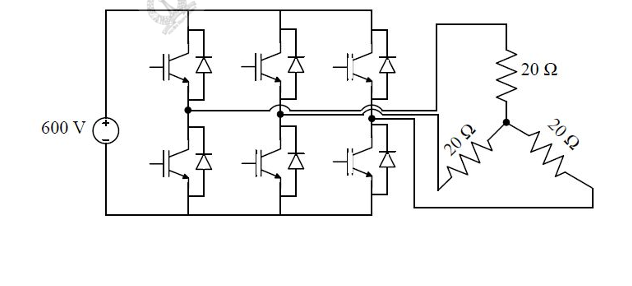
\includegraphics[width=0.5\columnwidth]{figs/25.png}
    \caption{}
    \label{fig:placeholder}
\end{figure}

\item A function $f(x)$ is defined as
\begin{align*}
    f(x) = \begin{cases}
e^x, & x < 1 \\
\ln x + x^n, & x \geq 1
\end{cases}
\end{align*}
where $x \in \mathbb{R}$. Which one of the following statements is TRUE?
\begin{enumerate}
\item $f(x)$ is NOT differentiable at $x=1$ for any values of $n$ and $b$.
\item $f(x)$ is differentiable at $x=1$ for the unique values of $n$ and $b$.
\item $f(x)$ is differentiable at $x=1$ for all values of $n$ and $b$ such that $b \neq e$.
\item $f(x)$ is differentiable at $x=1$ for all values of $n$ and $b$.
\end{enumerate}

\item Consider the differential equation
\begin{align*}
    (y^2 - 8)\frac{d^2y}{dx^2} - 5y\frac{dy}{dx} = x^3y, \quad y(0)=2.
\end{align*}
There exists a unique solution for this differential equation when $x$ belongs to the interval:
\begin{enumerate}
\begin{multicols}{4}
\item $(-2,2)$
\item $(0,10)$
\item $(-\infty,10)$
\item $(0,2)$
\end{multicols}
\end{enumerate}

\item Consider the line integral 
\begin{align*}
    I = \int_C (x^2y \, dx + y^2 \, dy), \quad C: \text{ from } (0,0) \to (1,1).
\end{align*}
\begin{figure}[H]
    \centering
    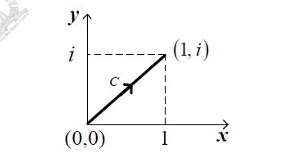
\includegraphics[width=0.5\columnwidth]{figs/28.png}
    \caption{}
    \label{fig:placeholder}
\end{figure}
The value of $I$ is:
\begin{enumerate}
\begin{multicols}{4}
    
\item $\tfrac{1}{2}$
\item $\tfrac{2}{3}$
\item $\tfrac{3}{4}$
\item $\tfrac{4}{3}$
\end{multicols}

\end{enumerate}



\item Two passive two-port networks are connected in cascade as shown in figure.  
A voltage source is connected at port 1.

\begin{figure}[H]
     \centering
     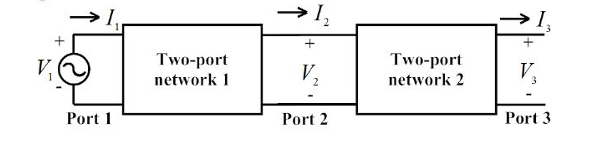
\includegraphics[width=0.5\columnwidth]{figs/29.png}
     \caption{}
     \label{fig:placeholder}
 \end{figure} 

Given
\begin{align*}
V_1 &= A_1 V_2 + B_1 I_2 \\
I_1 &= C_1 V_2 + D_1 I_2 \\
V_2 &= A_2 V_3 + B_2 I_3 \\
I_2 &= C_2 V_3 + D_2 I_3
\end{align*}
$A_1,B_1,C_1,D_1,A_2,B_2,C_2,D_2$ are generalized circuit constants.  
If Thevenin equivalent circuit at port 3 consists of voltage source $V_T$ and impedance $Z_T$ in series, then
\begin{enumerate}
\begin{multicols}{2}
    

\item $V_T = \tfrac{V_1}{A_1A_2+B_1C_2}, \quad Z_T = \tfrac{A_1B_2+B_1D_2}{A_1A_2+B_1C_2}$
\item $V_T = \tfrac{V_1}{A_1A_2+B_1C_2}, \quad Z_T = \tfrac{A_1B_2+B_1D_2}{A_1A_2+B_1C_2}$
\item $V_T = \tfrac{V_1}{A_1A_2+B_1C_2}, \quad Z_T = \tfrac{A_1B_2+B_1D_2}{A_1A_2+B_1C_2}$
\item $V_T = \tfrac{V_1}{A_1A_2+B_1C_2}, \quad Z_T = \tfrac{A_1B_2+B_1D_2}{A_1A_2+B_1C_2}$
\end{multicols}
\end{enumerate}


\item Let a causal LTI system be characterized by
\begin{figure}[H]
    \centering
    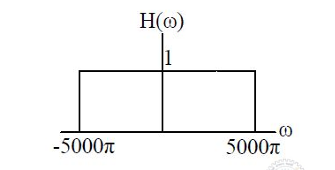
\includegraphics[width=0.5\columnwidth]{figs/31.png}
    \caption{}
    \label{fig:placeholder}
\end{figure}
\begin{align*}
\frac{d^2 y}{dt^2} + \frac{dy}{dt} + 10y(t) 
= 4x(t) + \frac{dx}{dt},
\end{align*}
with initial rest condition, where $x(t)$ is input and $y(t)$ is output.  
The impulse response of the system is
\begin{enumerate}
\item $2e^{-2t}u(t) - 7e^{-5t}u(t)$
\item $-2e^{-2t}u(t) + 7e^{-5t}u(t)$
\item $7e^{-2t}u(t) - 2e^{-5t}u(t)$
\item $-7e^{-2t}u(t) + 2e^{-5t}u(t)$
\end{enumerate}


\item Let the signal 
\[
x(t) = \sum_{k=-\infty}^{+\infty} (-1)^k \, \delta\left(t - \frac{k}{2000}\right)
\]
be passed through an LTI system with frequency response $H(\omega)$, as given in the figure below.  

The Fourier series representation of the output is given as  

\begin{multicols}{2}
\begin{enumerate}
\item $4000 + 4000\cos(2000\pi t) + 4000\cos(4000\pi t)$
\item $8000 + 2000\cos(2000\pi t) + 2000\cos(4000\pi t)$
\item $4000\cos(2000\pi t)$
\item $2000\cos(2000\pi t)$
\end{enumerate}
\end{multicols}

\item In the system whose signal flow graph is shown in the figure, $U_1(s)$ and $U_2(s)$ are the inputs. The transfer function $\dfrac{Y(s)}{U_1(s)}$ is  
\begin{figure}[H]
    \centering
    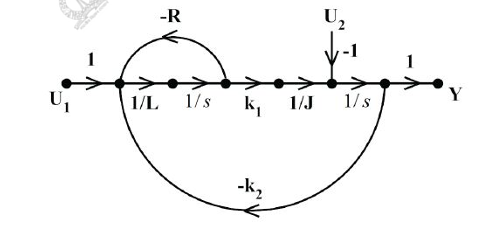
\includegraphics[width=0.5\columnwidth]{figs/32.png}
    \caption{}
    \label{fig:placeholder}
\end{figure}
\begin{multicols}{2}
\begin{enumerate}
\item $\dfrac{k_1}{JLs^2+Rs+k_1k_2}$
\item $\dfrac{k_1}{JLs^2 - Rs - k_1k_2}$
\item $\dfrac{k_1U_1(R+sL)}{JLs^2+UR-U_2Js+k_2U_2R}$
\item $\dfrac{k_1U_2(sL-R)}{JLs^2-(UR+U_2L)s-k_1k_2+U_2R}$
\end{enumerate}
\end{multicols}

\item The transfer function of the system $\dfrac{Y(s)}{U(s)}$ whose state-space equations are given below is:  

\[
\myvec{ \dot{x}_1(t) \\ \dot{x}_2(t) }
= \myvec{ 1 & 2 \\ -1 & 0 } 
\myvec{ x_1(t) \\ x_2(t) }
+ \myvec{ 1 \\ 1 } u(t),
\qquad
y(t) = \myvec{ 1 & 0 } 
\myvec{ x_1(t) \\ x_2(t) }
\]

\begin{multicols}{2}
\begin{enumerate}
\item $\dfrac{s+2}{(s+2)(s-4)}$
\item $\dfrac{s}{(s+2)(s-4)}$
\item $\dfrac{(s+2)}{(s+4)(s-2)}$
\item $\dfrac{(s+2)}{(s^2-s-4)}$
\end{enumerate}
\end{multicols}

\item The load shown in the figure is supplied by a 400 V (line-to-line), 3-phase source (RYB sequence). The load is balanced and inductive, drawing 3464 VA. When the switch $S$ is in position X, the three watt-meters $W_1, W_2, W_3$ read 577.35 W each. If the switch is moved to position Y, the readings of the watt-meters in watts will be:  
\begin{figure}[H]
    \centering
    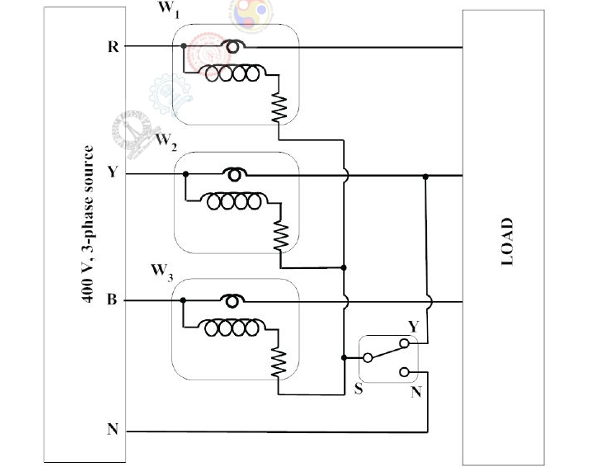
\includegraphics[width=0.5\columnwidth]{figs/34.png}
    \caption{}
    \label{fig:placeholder}
\end{figure}
\begin{multicols}{2}
\begin{enumerate}
\item $W_1 = 1732, \; W_2 = W_3 = 0$
\item $W_1 = 0, \; W_2 = 1732, \; W_3 = 0$
\item $W_1 = 0, \; W_2 = 0, \; W_3 = 1732$
\item $W_1 = W_2 = W_3 = 577.35$
\end{enumerate}
\end{multicols}




\item The approximate transfer characteristic for the circuit shown below with an ideal operational amplifier and diode will be:  

\begin{figure}[H]
    \centering
    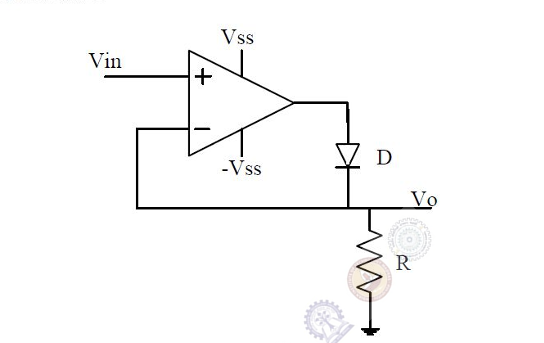
\includegraphics[width=0.5\columnwidth]{figs/35.png}
    \caption{}
    \label{fig:placeholder}
\end{figure}


\begin{enumerate}
\item 
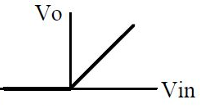
\includegraphics[width=0.5\columnwidth]{figs/35-a.png}
    \label{fig:placeholder}

\item 
 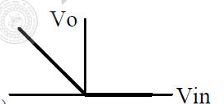
\includegraphics[width=0.5\columnwidth]{figs/35-b.png}

    \label{fig:placeholder}

\item 
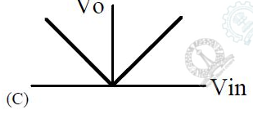
\includegraphics[width=0.5\columnwidth]{figs/35-c.png}
 
    \label{fig:placeholder}

\item 

    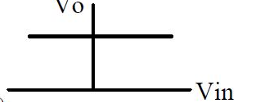
\includegraphics[width=0.5\columnwidth]{figs/35-d.png}
 
    \label{fig:placeholder}

\end{enumerate}


\item The output expression for the Karnaugh map shown below is:  

\begin{figure}[H]
    \centering
    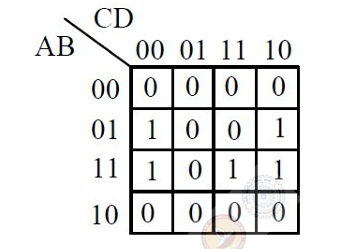
\includegraphics[width=0.5\columnwidth]{figs/36.png}
    \caption{}
    \label{fig:placeholder}
\end{figure}

\begin{multicols}{2}
\begin{enumerate}
\item $\overline{B}D + BCD$
\item $\overline{B}D + AB$
\item $\overline{B}D + ABC$
\item $\overline{B}D + ABC$
\end{enumerate}
\end{multicols}

\item The logical gate implemented using the circuit shown below, where $V_1$ and $V_2$ are inputs (with 0 V as digital 0 and 5 V as digital 1) and $V_{OUT}$ is the output, is:  

\begin{figure}[H]
    \centering
    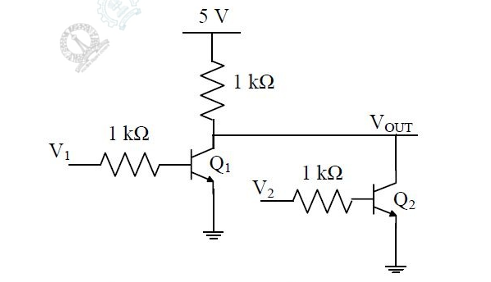
\includegraphics[width=0.5\columnwidth]{figs/37.png}
    \caption{}
    \label{fig:placeholder}
\end{figure}

\begin{multicols}{2}
\begin{enumerate}
\item NOT
\item NOR
\item NAND
\item XOR
\end{enumerate}
\end{multicols}

\item The input voltage $V_{DC}$ of the buck-boost converter shown below varies from 32 V to 72 V.  
Assume that all components are ideal, inductor current is continuous, and output voltage is ripple free. 
\begin{figure}[H]
    \centering
    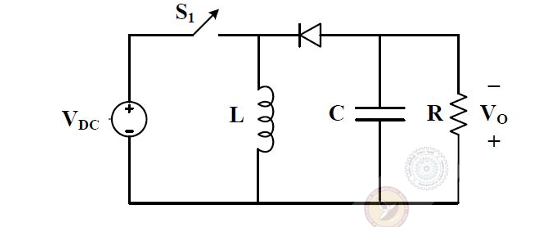
\includegraphics[width=0.5\columnwidth]{figs/38.png}
    \caption{}
    \label{fig:placeholder}
\end{figure}
The range of duty ratio $D$ of the converter for which the magnitude of the steady-state output voltage remains constant at 48 V is:  



\begin{multicols}{2}
\begin{enumerate}
\item $\tfrac{2}{3} \leq D \leq \tfrac{3}{4}$
\item $\tfrac{2}{5} \leq D \leq \tfrac{3}{5}$
\item $0 \leq D \leq 1$
\item $\tfrac{1}{3} \leq D \leq \tfrac{2}{3}$
\end{enumerate}
\end{multicols}

\item A load is supplied by a 230 V, 50 Hz source. The active power $P$ and the reactive power $Q$ consumed by the load are such that $1 \,\text{kW} \leq P \leq 2 \,\text{kW}$ and $1 \,\text{kVAR} \leq Q \leq 2 \,\text{kVAR}$. A capacitor connected across the load for power factor correction generates 1 kVAR reactive power. The worst case power factor after power factor correction is:  

\begin{multicols}{2}
\begin{enumerate}
\item 0.447 lag
\item 0.707 lag
\item 0.894 lag
\item 1
\end{enumerate}
\end{multicols}

\item The bus admittance matrix for a power system network is:  

\[
\myvec{
-39.9 & j20 & j20 \\
j20 & -39.9 & j20 \\
j20 & j20 & -39.9
} \, \text{pu}
\]

There is a transmission line, connected between buses 1 and 3, represented by the circuit shown below.  
Reactance is 0.05 pu, susceptance is 0.05 pu.  
\begin{figure}[H]
    \centering
    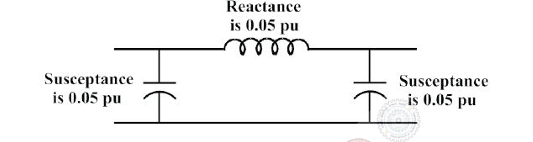
\includegraphics[width=0.5\columnwidth]{figs/40.png}
    \caption{}
    \label{fig:placeholder}
\end{figure}

If this transmission line is removed from service, the modified bus admittance matrix is:  

\begin{multicols}{2}
\begin{enumerate}
\item $\myvec{-19.9 & j20 & 0 \\ j20 & -39.9 & j20 \\ 0 & j20 & -19.95}$
\item $\myvec{-39.95 & j20 & 0 \\ j20 & -39.9 & j20 \\ 0 & j20 & -39.95}$
\item $\myvec{-19.95 & j20 & 0 \\ j20 & -39.9 & j20 \\ 0 & j20 & -19.95}$
\item $\myvec{-19.95 & j20 & 0 \\ j20 & -39.9 & j20 \\ 0 & j20 & -19.95}$
\end{enumerate}
\end{multicols}

\item The switch in the figure below was closed for a long time. It is opened at $t=0$.  
The current in the inductor of 2 H for $t \geq 0$ is:  
\begin{figure}[H]
    \centering
    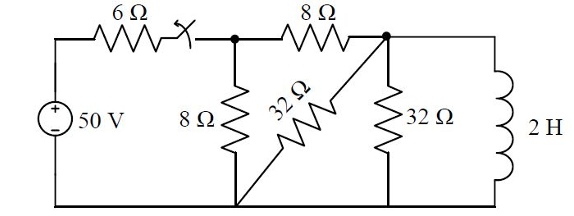
\includegraphics[width=0.5\columnwidth]{figs/41.png}
    \caption{}
    \label{fig:placeholder}
\end{figure}


\begin{multicols}{2}
\begin{enumerate}
\item $2.5 e^{-4t}$
\item $5 e^{-4t}$
\item $2.5 e^{-0.25t}$
\item $5 e^{-0.25t}$
\end{enumerate}
\end{multicols}



\item Only one of the real roots of 
\begin{align*}
    f(x) = x^6 - x - 1
\end{align*}
lies in the interval \(1 \leq x \leq 2\) and bisection method is used to find its value. For achieving an accuracy of \(0.001\), the required minimum number of iterations is \underline{\hspace{2cm}}.

\item In the circuit shown below, the maximum power transferred to the resistor \(R\) is \underline{\hspace{2cm}} W.  

\begin{figure}[H]
    \centering
    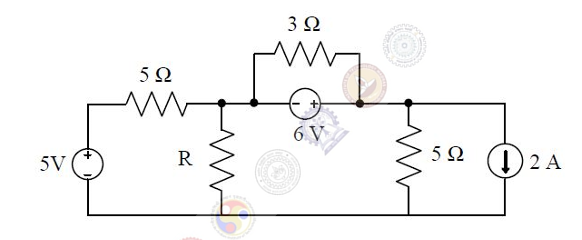
\includegraphics[width=0.5\columnwidth]{figs/43.png}
    \caption{}
    \label{fig:placeholder}
\end{figure}


\item The magnitude of magnetic flux density \((B)\) in micro Teslas (\(\mu T\)), at the center of a loop of wire wound as a regular hexagon of side length \(1\,m\) carrying a current \(I=1\,A\), and placed in vacuum as shown in the figure is \underline{\hspace{2cm}}.  
(Give the answer up to two decimal places.)  

\begin{figure}[H]
    \centering
    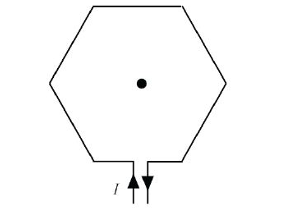
\includegraphics[width=0.5\columnwidth]{figs/44.png}
    \caption{}
    \label{fig:placeholder}
\end{figure}


\item A \(375 \, W, \, 230 \, V, \, 50 \, Hz\) capacitor start single-phase induction motor has the following constants for the main and auxiliary windings (at starting):  
\begin{align*}
    Z_m = (12.50 + j15.75)\,\Omega \quad (\text{main winding}),
\end{align*}
\begin{align*}
    Z_a = (24.50 + j12.75)\,\Omega \quad (\text{auxiliary winding}).
\end{align*}
Neglecting the magnetizing branch, the value of the capacitance (in \(\mu F\)) to be added in series with the auxiliary winding to obtain maximum torque at starting is \underline{\hspace{2cm}}.


\item Two parallel connected, three-phase, 50Hz, 11 kV, star-connected synchronous machines A and B are operating as synchronous condensers. They together supply \(50 \, MVAR\) to a \(11\,kV\) grid. Current supplied by both the machines are equal. Synchronous reactances of machine A and B are \(1 \, \ohm\) and \(3 \, \ohm\), respectively.  
Assuming the magnetic circuit to be linear, the ratio of exciting current of machine A to that of machine B is \underline{\hspace{2cm}}.  
(Give the answer up to two decimal places.)


\item A \(220 \, V\) DC series motor runs drawing a current of \(30 \, A\) from the supply. Armature and field circuit resistances are \(0.4 \, \ohm\) and \(0.1 \, \ohm\), respectively. The load torque varies as the square of the speed. The flux in the motor may be taken as being proportional to the armature current. To reduce the speed of the motor by \(50\%\), the resistance in ohms that should be added in series with the armature is \underline{\hspace{2cm}}.  
(Give the answer up to two decimal places.)


\item A three-phase, three winding \(\Delta/Y/ (11\,kV/6.6\,kV/400\,V)\) transformer is energized from AC mains at the \(11 \, kV\) side. It supplies \(900 \, kVA\) load at 0.8 power factor lag from the \(6.6 \, kV\) winding and \(300 \, kVA\) load at 0.6 power factor lag from the \(400 \, V\) winding. The RMS line current in ampere drawn by the \(11\,kV\) winding from the mains is \underline{\hspace{2cm}}.  
(Give the answer up to one decimal place.)


\item A separately excited DC generator supplies \(150 \, A\) to a \(145 \, V\) DC grid. The generator is running at 800 RPM. The armature resistance of the generator is \(0.1 \ohm\). If the speed of the generator is increased to 1000 RPM, the current in amperes supplied by the generator to the DC grid is \underline{\hspace{2cm}}.  
(Give the answer up to one decimal place.)


\item For a system having transfer function  
\begin{align*}
    G(s) = \frac{-s+1}{s+1},
\end{align*}
a unit step input is applied at time \(t=0\). The value of the response of the system at \(t=1.5 \, sec\) (rounded off to three decimal places) is \underline{\hspace{2cm}}.


\item Consider a causal and stable LTI system with rational transfer function \(H(z)\), whose corresponding impulse response begins at \(n=0\). Furthermore, \(H(1) = \frac{5}{4}\).  
The poles of \(H(z)\) are 
\begin{align*}
    p_k = \frac{1}{2} \exp\Big( j \frac{(2k-1)\pi}{4}\Big), \quad k=1,2,3,4.
\end{align*}
The zeros of \(H(z)\) are all at \(z=0\). Let \(g[n] = r^n h[n]\). The value of \(g[8]\) equals \underline{\hspace{2cm}}.  
(Give the answer up to three decimal places.)


\item The circuit shown in the figure uses matched transistors with a thermal voltage \(V_T = 25\, mV\). The base currents of the transistors are negligible. The value of the resistance \(R\) in \(k\ohm\) that is required to provide \(1\, \mu A\) bias current for the differential amplifier block shown is \underline{\hspace{2cm}}.  
(Give the answer up to one decimal place.)  

\begin{figure}[H]
    \centering
    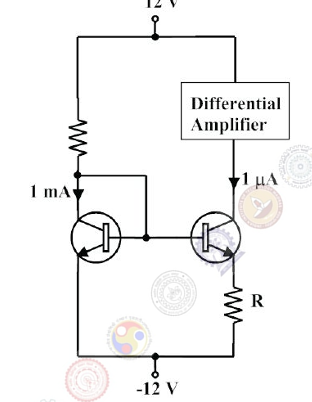
\includegraphics[width=0.5\columnwidth]{figs/52.png}
    \caption{}
    \label{fig:placeholder}
\end{figure}


\item The figure below shows an uncontrolled diode bridge rectifier supplied from a \(220 \, V, \, 50\, Hz\), single-phase source. The load draws a constant current \(I_0 = 14 \, A\). The conduction angle of the diode \(D_1\), in degrees (rounded off to two decimal places) is \underline{\hspace{2cm}}.  

\begin{figure}[H]
    \centering
    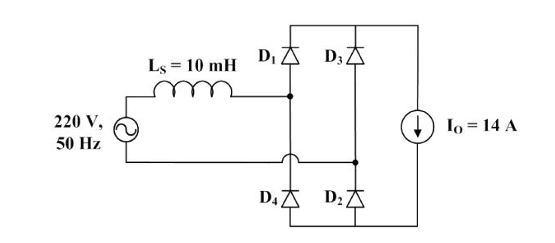
\includegraphics[width=0.5\columnwidth]{figs/54.png}
    \caption{}
    \label{fig:placeholder}
\end{figure}



\item The positive, negative, and zero sequence reactances of a wye-connected synchronous generator are 0.2 pu, 0.2 pu, and 0.1 pu, respectively. 
The generator is on open circuit with a terminal voltage of 1 pu. 
The minimum value of the inductive reactance, in pu, required to be connected between neutral and ground so that the fault current does not exceed 3.75 pu if a single line to ground fault occurs at the terminals is \\\\\_ (assume fault impedance to be zero).  
(Give the answer up to one decimal place.)


\item The figure shows the single line diagram of a power system with a double circuit transmission line. The expression for electrical power is 
\begin{figure}[H]
    \centering
    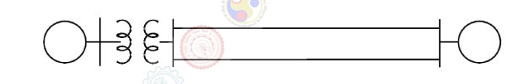
\includegraphics[width=0.5\columnwidth]{figs/55.png}
    \caption{}
    \label{fig:placeholder}
\end{figure}
\begin{align*}
P = 1.5 \sin \delta
\end{align*}
where $\delta$ is the rotor angle.  
The system is operating at stable equilibrium point with mechanical power (input) $P_m = 1.0$ pu.  
If one of the transmission circuits is removed, the maximum value of $\delta$ at the rotor swings is $121.1^\circ$.  
The maximum value of electrical power with one transmission line circuit removed is $P_{\max} = 0.85$ pu.  
The value of $P_m$ in pu is \\\\\_ (Give the answer up to three decimal places.)


\item After Rajendra Chola returned from his voyage to Indonesia, he \\\\\_ to visit the temple in Thanjavur.
\begin{multicols}{2}
\begin{enumerate}
\item was wishing  
\item is wishing  
\item wished  
\item had wished  
\end{enumerate}
\end{multicols}


\item Research in the workplace reveals that people work for many reasons
\begin{multicols}{2}
\begin{enumerate}
\item money beside  
\item beside money  
\item money besides  
\item besides money  
\end{enumerate}
\end{multicols}


\item Rahul, Murali, Srinivas and Anil are seated around a square table.  
Rahul is sitting to the left of Murali. Srinivas is sitting to the right of Anil.  
Which of the following pairs are seated opposite each other?
\begin{multicols}{2}
\begin{enumerate}
\item Rahul and Murali  
\item Srinivas and Anil  
\item Srinivas and Murali  
\item Srinivas and Rahul  
\end{enumerate}
\end{multicols}


\item Find the smallest number $y$ such that $y \times 162$ is a perfect cube.
\begin{multicols}{2}
\begin{enumerate}
\item 24  
\item 27  
\item 32  
\item 36  
\end{enumerate}
\end{multicols}


\item The probability that a $k$-digit number does NOT contain the digits 0, 5, or 9 is
\begin{multicols}{2}
\begin{enumerate}
\item $0.3^k$  
\item $0.6^k$  
\item $0.7^k$  
\item $0.9^k$  
\end{enumerate}
\end{multicols}


\item ``The hold of the nationalist imagination on our colonial past is such that anything inadequately or improperly nationalist is just not history.''  
Which of the following statements best reflects the author's opinion?
\begin{multicols}{2}
\begin{enumerate}
\item Nationalists are highly imaginative.  
\item History is viewed through the filter of nationalism.  
\item Our colonial past never happened.  
\item Nationalism has to be both adequately and properly imagined.  
\end{enumerate}
\end{multicols}


\item Six people are seated around a circular table. There are at least three men and two women. There are at least three right-handed persons.  
Every woman has a left-handed person to her immediate right. None of the women are right-handed.  
The number of women at the table is
\begin{multicols}{2}
\begin{enumerate}
\item 2  
\item 3  
\item 4  
\item Cannot be determined  
\end{enumerate}
\end{multicols}


\item The expression 
\begin{align*}
\frac{(x+y) - |x-y|}{2}
\end{align*}
is equal to
\begin{multicols}{2}
\begin{enumerate}
\item the maximum of $x$ and $y$  
\item the minimum of $x$ and $y$  
\item 1  
\item none of the above  
\end{enumerate}
\end{multicols}


\item Arun, Gulab, Neel and Shweta must choose one shirt each from a pile of four shirts coloured red, pink, blue and white respectively.  
Arun dislikes the colour red and Shweta dislikes the colour white.  
Gulab and Neel like all the colours.  
In how many different ways can they choose the shirts so that no one has a shirt with a colour he or she dislikes?
\begin{multicols}{2}
\begin{enumerate}
\item 21  
\item 18  
\item 16  
\item 14  
\end{enumerate}
\end{multicols}


\item A contour line joins locations having the same height above the mean sea level.  
The following is a contour plot of a geographical region.  
\begin{figure}[H]
    \centering
    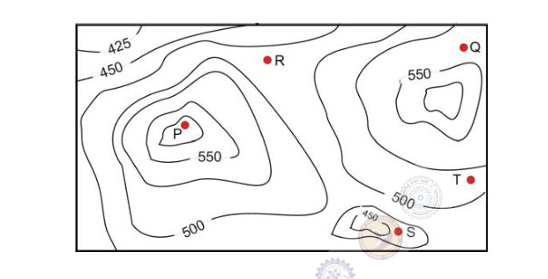
\includegraphics[width=0.5\columnwidth]{figs/65.png}
    \caption{}
    \label{fig:placeholder}
\end{figure}
Contour lines are shown at 25 m intervals in this plot.  
If in a flood, the water level rises to 525 m, which of the villages P, Q, R, S, T get submerged?
\begin{multicols}{2}
\begin{enumerate}
\item P, Q  
\item P, Q, T  
\item R, S, T  
\item Q, R, S  
\end{enumerate}
\end{multicols}

\end{enumerate}
\end{document}

